\documentclass[newpage,hints,12pt,nooutcomes,noauthor,handout]{ximera}

%\usepackage{microtype}
%\usepackage{tikz}
\usepackage{tkz-euclide}
%\usetkzobj{all}
\tikzstyle geometryDiagrams=[rounded corners=.5pt,ultra thick,color=blue!50!black]

\usepackage{tikz-cd}

\colorlet{penColor}{blue!50!black} % Color of a curve in a plot

%% \hypersetup{
%%     colorlinks = false,
%%     }


\tikzset{%% partial ellipse
    partial ellipse/.style args={#1:#2:#3}{
        insert path={+ (#1:#3) arc (#1:#2:#3)}
    }
}

\graphicspath{
{./}
{sphericalLunesAndTriangles/}
{hyperbolicLunesAndTriangles/}
{centralProjection/}
{stereographicProjection/}
{linesAnglesAndAreasInCentralProjection/}
{linesAnglesAndAreasInStereographicProjection/}
{stereographicProjection/}
{centralProjectionInHG/}
{stereographicProjectionInHG/}
{linesInSphericalGeometry/}
{linesInHyperbolicGeometry/}
{theArtOfEscher/}
}


\newcommand{\transpose}{\intercal}
\newcommand{\eval}[1]{\bigg[ #1 \bigg]}

\renewcommand{\epsilon}{\varepsilon}
\renewcommand{\l}{\ell}
\renewcommand{\d}{\,d}

\DeclareMathOperator{\arccosh}{arccosh}
\DeclareMathOperator{\arctanh}{arctanh}
\renewcommand{\tilde}{\widetilde}
\newcommand{\R}{\mathbb R}
\newcommand{\dd}[2][]{\frac{d #1}{d #2}}
\newcommand{\pp}[2][]{\frac{\partial #1}{\partial #2}}
\newcommand{\dfn}{\textbf}

\renewcommand{\bar}{\overline}
\renewcommand{\hat}{\widehat}


\ifxake
\NewEnviron{freeResponse}{}
\fi


\title{Hyperbolic lunes and triangles}

\begin{document}
\begin{abstract}
In this activity, we explore the areas of lunes and triangles in
hyperbolic geometry.
\end{abstract}
\maketitle

We know that the area of a triangle on the $R$-sphere with angles
$\alpha$, $\beta$, and $\gamma$ is given by
\[
R^2(\alpha+\beta+\gamma - \pi).
\]

\begin{problem}
  Briefly sketch the line of reasoning used to deduce the formula for
  the area of a triangle on the $R$-sphere.
\end{problem}

We will use similar reasoning to deduce the formula for the area of a triangle
with angles $\alpha$, $\beta$, and $\gamma$ in hyperbolic geometry.

\subsection{Hyperbolic lunes}

Consider the following diagram on the Klein disk, that is the central projection
of hyperbolic geometry:
%% \begin{image}
%%   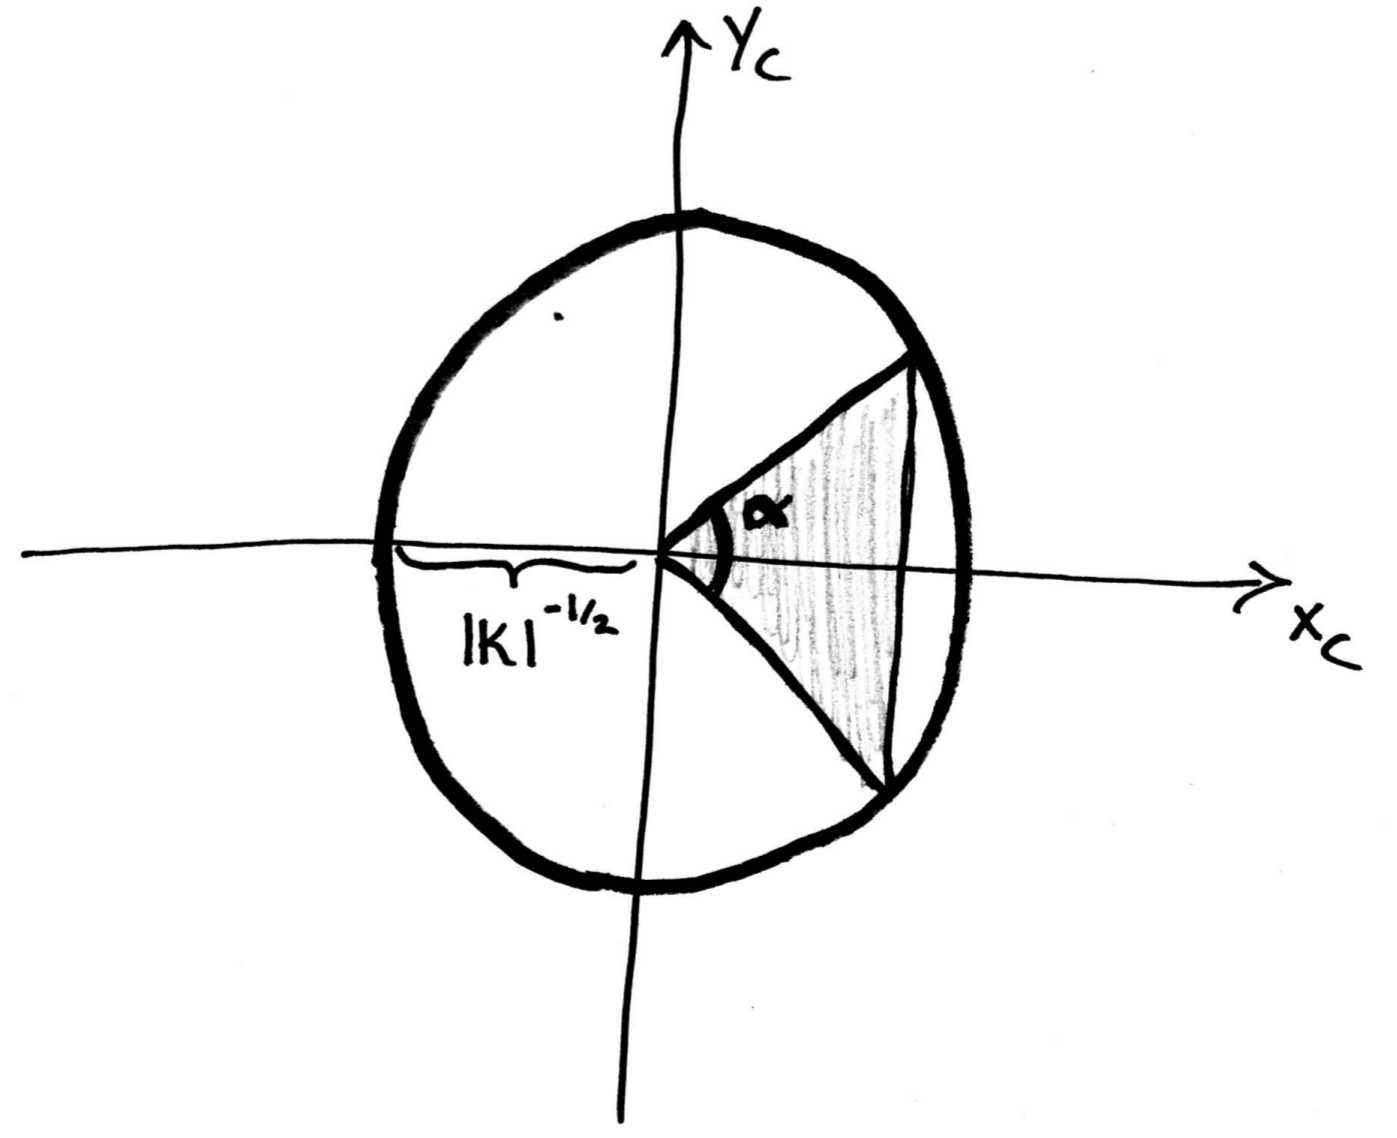
\includegraphics[width=3in]{diagramOfHyperbolicLune.png}
%% \end{image}
\begin{center}
\begin{tikzpicture}[geometryDiagrams,scale=3]
    \tkzDefPoint(0,0){O}
    \tkzDefPoint(1,0){A}
    %\tkzDrawCircle[ultra thick,fill=black!10!white](O,A)
    \tkzDrawCircle(O,A)
    \draw[ultra thick, fill = black!10!white] (0,0)--({cos(30)},{sin(30)})--({cos(-30)},{sin(-30)})--cycle;
    
  %% x_s-axis
  \draw [thin,->] (-1.2,0)--(1.2,0); 
  \node[right] at (1.2,0) {$x_c$};
  
  %% y_s-axis
  \draw [thin,->] (0,-1.2)--(0,1.2); 
  \node[above] at (0,1.2) {$y_c$};

  
  
  \draw [
    thin,
    decoration={
        brace,
        raise=0.1cm
    },
    decorate
  ] (-.03,0) -- (-.97,0) node [pos=0.5,anchor=north,yshift=-0.1cm] {$|K|^{-1/2}$};


  \draw[thick] (.3,0) arc (0:30:.3);
  \draw[thick] (.3,0) arc (0:-30:.3);
  \node at (.2,.05) {$\alpha$};
\end{tikzpicture}
\end{center}



Notice that in both the Klein model and the Poincar\'e model, every line hits
``the circle at infinity'' at two specific points.  This means we can talk about
shapes with ``vertices at infinity''.

\begin{definition}
  We define an \dfn{$\boldsymbol\alpha$-lune} in hyperbolic geometry to be a
  triangle with an angle of measure $\alpha$ where vertices opposite of $\alpha$
  are at infinity.
\end{definition}

We have seen that to compute areas in central projection, we use
\[
  \iint_{L_c} \sqrt{\det P_c}\d x_c\d y_c
  =\iint_{L_c} \left(K\left(x_c^2+y_c^2\right)+1\right)^{-3/2} \d x_c\d y_c.
\]


In what follows, we will assume that $K=-1$. This will simplify the
computations somewhat. Once the mathematician is familiar with this
case, the general case when $K<0$ will fall easily.


\begin{problem}
  Convert
  \[
  \iint_{L_c} \left(-\left(x_c^2+y_c^2\right)+1\right)^{-3/2} \d x_c\d y_c
  \]
  to polar coordinates and compute the integral.
  \begin{hint}
    Redraw the picture above with $\alpha = 2\beta$ and $K=-1$.
  \end{hint}
  \begin{hint}
    Recall that to convert to polar coordinates, set
    \begin{align*}
      r &= \sqrt{x_c^2+y_c^2},\\
      \theta &= \arctan(y_c/x_c),
    \end{align*}
    and replace $\d x_c\d y_c$ with $r\d r\d \theta$.
  \end{hint}
  \begin{hint}
    At some point you may wish to use the following identities:
    \[
    \begin{split}
      \cos^2\theta + \sin^2\theta &=1\\
      \cos^2\theta &= 1-\sin^2\theta
    \end{split}
    \qquad
    \begin{split}
      \cos^2\beta + \sin^2\beta &=1\\
      \cos^2\beta &= 1-\sin^2\beta
    \end{split}
    \]
    So
    \begin{align*}
      \cos^2\theta - \cos^2\beta &= 1 - \sin^2\theta - \left(1-\sin^2\beta\right)\\
      &= \sin^2\beta - \sin^2\theta.       
    \end{align*}
  \end{hint}
  \begin{hint}
    It may also be helpful to recall that when $a>0$,
    \[
    \int \frac{1}{\sqrt{a - u^2}} \d u = \arcsin\left(\frac{u}{\sqrt{a}}\right) + C.
    \]
  \end{hint}
  \begin{hint}
    Finally, as a gesture of friendship, I will tell you that you will
    (hopefully!) deduce that this integral equals $\pi-\alpha$.
  \end{hint}
  \begin{freeResponse}
    Write
    \[
    \int_{L_c} \left(-\left(x_c^2+y_c^2\right)+1\right)^{-3/2} \d x_c\d y_c
    = \int_{-\beta}^\beta \int_0^{\frac{\cos \beta}{\cos\theta}}\left(-r^2+1\right)^{-3/2} r\d r\d \theta.
    \]
    Integrating this from the inside-out we find
    \begin{align*}
      &= \int_{-\beta}^\beta \eval{\left(-r^2+1\right)^{-1/2}}_0^{\frac{\cos \beta}{\cos\theta}}\d \theta\\
      &= \int_{-\beta}^\beta \left(-\left(\frac{\cos \beta}{\cos\theta}\right)^2+1\right)^{-1/2}\d\theta - \eval{\theta}_{-\beta}^\beta\\
      &= \int_{-\beta}^\beta \left(1-\frac{\cos^2 \beta}{\cos^2\theta}\right)^{-1/2}\d \theta -2\beta\\
      &= \int_{-\beta}^\beta \left(\frac{\cos^2\theta - \cos^2 \beta}{\cos^2\theta}\right)^{-1/2} \d \theta-\alpha\\
      &= \int_{-\beta}^\beta \frac{\cos\theta}{\sqrt{\cos^2\theta - \cos^2 \beta}}\d \theta - \alpha.
    \end{align*}
    Now apply a trigonometric substitution,
    \[
    = \int_{-\beta}^\beta \frac{\cos\theta}{\sqrt{\sin^2\beta - \sin^2 \theta}}\d \theta- \alpha,
    \]
    Using the hint above we see
    \begin{align*}
      &= \eval{\arcsin\left(\frac{\sin\theta}{\sin\beta}\right)}_{-\beta}^\beta - \alpha\\
      &= \arcsin\left(\frac{\sin\beta}{\sin\beta}\right)- \arcsin\left(\frac{\sin(-\beta)}{\sin\beta}\right)- \alpha\\
      &= \arcsin(1)-\arcsin(-1)-\alpha\\
      &= \frac{\pi}{2}-\frac{-\pi}{2}-\alpha\\
      &= \pi-\alpha.
    \end{align*}
  \end{freeResponse}
\end{problem}


\subsection{Hyperbolic triangles}

Again assuming $K=-1$, we will use our knowledge that the hyperbolic
$\alpha$-lune has area $\pi-\alpha$ to compute the area of an
\textit{ideal triangle} in hyperbolic geometry. Note, now we are
working under stereographic projection in the Poincar\'e disk, because
angles are preserved in the Poincar\'e disk.

\begin{definition}
  An \dfn{ideal triangle} is a triangle in hyperbolic geometry with all of
  its vertices at infinity.
\end{definition}

\begin{problem}
  Use the diagrams below
  %% \begin{image}
  %% 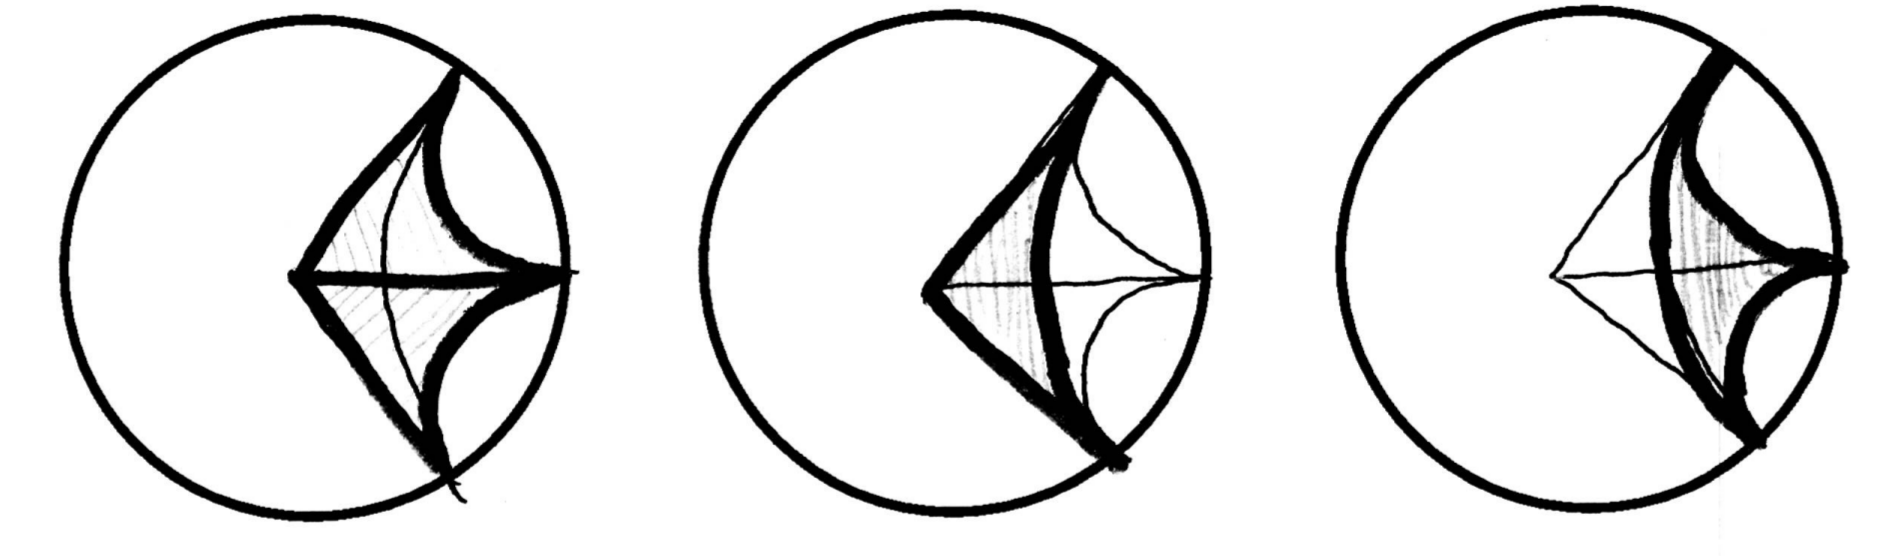
\includegraphics[width=4in]{diagramOfIdealTri.png}
  %% \end{image}
  \begin{center}
\begin{tikzpicture}[geometryDiagrams,scale=1.7]
  %% x_s-axis
  \draw [thin,->] (-1.2,0)--(1.2,0); 
  \node[right] at (1.2,0) {$x_s$};
  
  %% y_s-axis
  \draw [thin,->] (0,-1.2)--(0,1.2); 
  \node[above] at (0,1.2) {$y_s$};


  \tkzDefPoint(0,0){O}
  \tkzDefPoint(1,0){A}
  \tkzDrawCircle[thick](O,A)

  \tkzDefPoint(.5,.87){z1}
  \tkzDefPoint(.5,-.87){z2}

  \begin{scope}
    \clip (O) -- (z1) -- (A) -- (z2) -- cycle;
    \draw[fill = black!10!white, draw=none] (0,-1) rectangle (1,1);
  \end{scope}

  
  \tkzClipCircle(O,A)
  \tkzDrawCircle[fill=white,ultra thick,orthogonal through=A and z1](O,A)
  \tkzDrawCircle[fill=white,ultra thick,orthogonal through=A and z2](O,A)
  \tkzDrawCircle[orthogonal through=z1 and z2](O,A)
  \draw (O) -- (z1);
  \draw (O) -- (z2);
  \draw (O) -- (A);
  \tkzDrawCircle[thick](O,A)
  %\tkzDrawPoints[color=black,fill=black,size=5](z1)
  %\tkzDrawPoints[color=black,fill=black,size=5](z2)
\end{tikzpicture}
\begin{tikzpicture}[geometryDiagrams,scale=1.7]
  %% x_s-axis
  \draw [thin,->] (-1.2,0)--(1.2,0); 
  \node[right] at (1.2,0) {$x_s$};
  
  %% y_s-axis
  \draw [thin,->] (0,-1.2)--(0,1.2); 
  \node[above] at (0,1.2) {$y_s$};


  \tkzDefPoint(0,0){O}
  \tkzDefPoint(1,0){A}
  \tkzDrawCircle[thick](O,A)

  \tkzDefPoint(.5,.87){z1}
  \tkzDefPoint(.5,-.87){z2}


  \begin{scope}
    \clip (O) -- (z1) -- (A) -- (z2) -- cycle;
    \draw[fill = black!10!white, draw=none] (0,-1) rectangle (1,1);
  \end{scope}


  
  \tkzClipCircle(O,A)
  \tkzDrawCircle[fill=white,ultra thick,orthogonal through=z1 and z2](O,A)
  \tkzDrawCircle[thick,orthogonal through=A and z1](O,A)
  \tkzDrawCircle[thick,orthogonal through=A and z2](O,A)
  \draw (O) -- (z1);
  \draw (O) -- (z2);
  \draw[thick] (O) -- (A);

  \tkzDrawCircle[thick](O,A)
  %\tkzDrawPoints[color=black,fill=black,size=5](z1)
  %\tkzDrawPoints[color=black,fill=black,size=5](z2)
\end{tikzpicture}
\begin{tikzpicture}[geometryDiagrams,scale=1.7]
  %% x_s-axis
  \draw [thin,->] (-1.2,0)--(1.2,0); 
  \node[right] at (1.2,0) {$x_s$};
  
  %% y_s-axis
  \draw [thin,->] (0,-1.2)--(0,1.2); 
  \node[above] at (0,1.2) {$y_s$};


  \tkzDefPoint(0,0){O}
  \tkzDefPoint(1,0){A}
  \tkzDrawCircle[thick](O,A)

  \tkzDefPoint(.5,.87){z1}
  \tkzDefPoint(.5,-.87){z2}


   % \begin{scope}
   % \clip (O) -- (z1) -- (A) -- (z2) -- cycle;
   % \draw[fill = black!10!white, draw=none] (0,-1) rectangle (1,1);
  %\end{scope}
  
  \tkzClipCircle(O,A)
  \tkzDrawCircle[fill=black!10!white,ultra thick,orthogonal through=z1 and z2](O,A)
  \tkzDrawCircle[fill=white,ultra thick,orthogonal through=A and z1](O,A)
  \tkzDrawCircle[fill=white,ultra thick,orthogonal through=A and z2](O,A)

  \draw[thick] (O) -- (z1);
  \draw[thick] (O) -- (z2);
  \draw[thick] (O) -- (A);
  \tkzDrawCircle[thick](O,A)
  %\tkzDrawPoints[color=black,fill=black,size=5](z1)
  %\tkzDrawPoints[color=black,fill=black,size=5](z2)
\end{tikzpicture}
\end{center}

  to help compute the area of an ideal triangle in hyperbolic geometry.
  \begin{hint}
    Above we see a comic-strip of Poincar\'e disks.
  \end{hint}
  \begin{hint}
    Make sure your computation is general.  That is, start with an arbitrary
    ideal triangle and then fill in the rest of the diagram.
  \end{hint}
\end{problem}


\begin{definition}
  An \dfn{ideal $\boldsymbol{n}$-gon} is an $n$-gon in hyperbolic
  geometry with its vertices at infinity.
\end{definition}

%% \begin{problem}
%% Use induction to derive a formula for the area of any ideal $n$-gon in
%% hyperbolic geometry.
%% \end{problem}

\begin{problem}
  Use the diagrams below
  %% \begin{image}
  %% 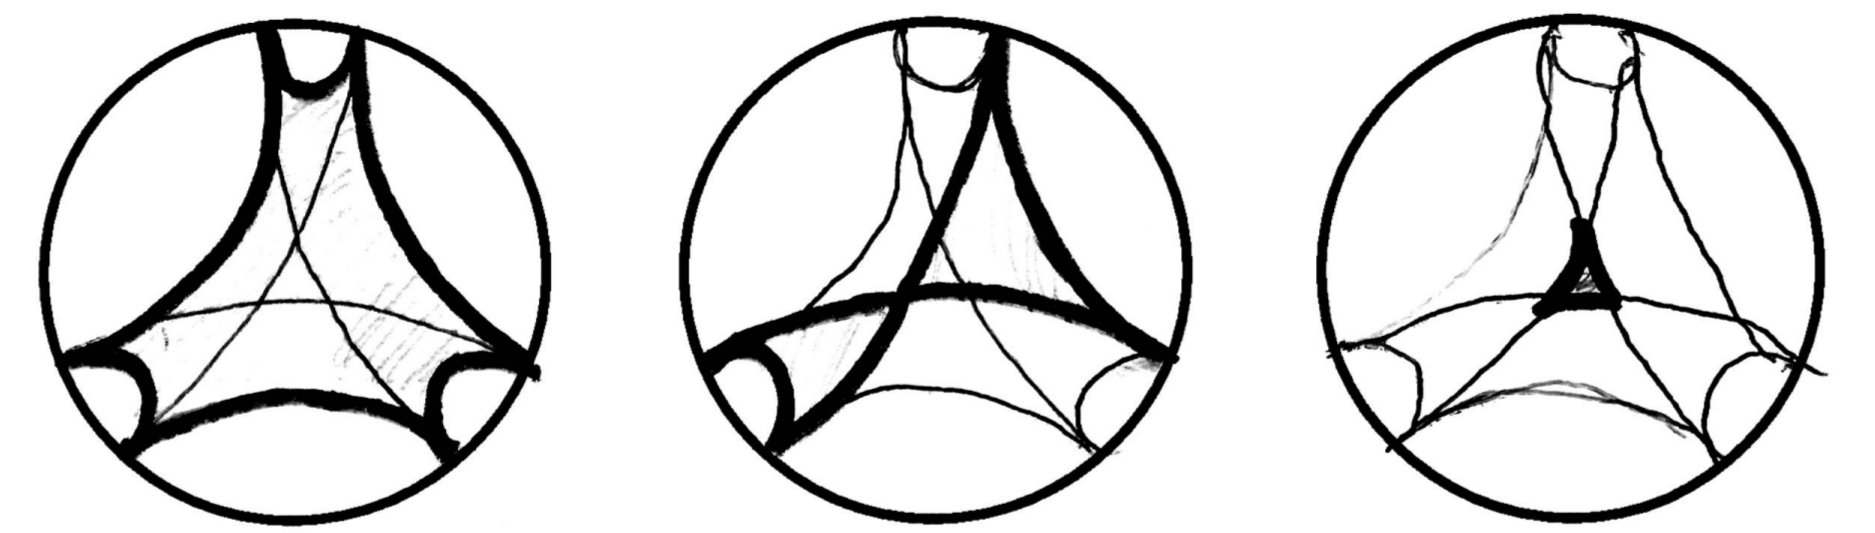
\includegraphics[width=4in]{diagramHex.png}
  %% \end{image}
  \begin{center}
\begin{tikzpicture}[geometryDiagrams,scale=1.7]
   %% x_s-axis
  \draw [thin,->] (-1.2,0)--(1.2,0); 
  \node[right] at (1.2,0) {$x_s$};
  
  %% y_s-axis
  \draw [thin,->] (0,-1.2)--(0,1.2); 
  \node[above] at (0,1.2) {$y_s$};
  \tkzDefPoint(0,0){O}
  \tkzDefPoint(1,0){A}
  \tkzDrawCircle[fill=black!10!white,thick](O,A)

  \tkzDefPoint(.3,.96){z1}
  \tkzDefPoint(-.3,.96){z2}

  \tkzDefPoint(-.98,-.22){z3}
  \tkzDefPoint(-.68,-.74){z4}

  \tkzDefPoint(.68,-.74){z5}
  \tkzDefPoint(.98,-.22){z6}
    
  \tkzClipCircle(O,A)
  \tkzDrawCircle[thick,orthogonal through=z1 and z3](O,A)
  \tkzDrawCircle[thick,orthogonal through=z3 and z5](O,A)
  \tkzDrawCircle[thick,orthogonal through=z5 and z1](O,A)
  \tkzDrawCircle[fill=white,ultra thick,orthogonal through=z1 and z2](O,A)
  \tkzDrawCircle[fill=white,ultra thick,orthogonal through=z2 and z3](O,A)
  \tkzDrawCircle[fill=white,ultra thick,orthogonal through=z3 and z4](O,A)
  \tkzDrawCircle[fill=white,ultra thick,orthogonal through=z4 and z5](O,A)
  \tkzDrawCircle[fill=white,ultra thick,orthogonal through=z5 and z6](O,A)
  \tkzDrawCircle[fill=white,ultra thick,orthogonal through=z6 and z1](O,A)
  
  

  \tkzDrawCircle[thick](O,A)
  %% x_s-axis
  \draw [thin,->] (-1.2,0)--(1.2,0); 
  \node[right] at (1.2,0) {$x_s$};
  
  %% y_s-axis
  \draw [thin,->] (0,-1.2)--(0,1.2); 
  \node[above] at (0,1.2) {$y_s$};
\end{tikzpicture}
\begin{tikzpicture}[geometryDiagrams,scale=1.7]
  %% x_s-axis
  \draw [thin,->] (-1.2,0)--(1.2,0); 
  \node[right] at (1.2,0) {$x_s$};
  
  %% y_s-axis
  \draw [thin,->] (0,-1.2)--(0,1.2); 
  \node[above] at (0,1.2) {$y_s$};


  \tkzDefPoint(0,0){O}
  \tkzDefPoint(1,0){A}
  \tkzDrawCircle[thick](O,A)
  
  \tkzDefPoint(.3,.96){z1}
  \tkzDefPoint(-.3,.96){z2}

  \tkzDefPoint(-.98,-.22){z3}
  \tkzDefPoint(-.68,-.74){z4}

  \tkzDefPoint(.68,-.74){z5}
  \tkzDefPoint(.98,-.22){z6}


  \tkzDefPoint(0,-.3){o1}
  
  \tkzClipCircle(O,A)
  \draw[fill=black!10!white,draw=none] (0,.15) -- (z5) -- (z4) -- cycle;
  \draw[fill=black!10!white,draw=none] (0,.2) -- (.1,.05) -- (-.1,.05) -- cycle;

  \draw[fill=black!10!white,draw=none] (0,.2) -- (z1) -- (z2) -- cycle;
  %\draw[fill=black!10!white,draw=none] (0,.2) -- (.1,.05) -- (-.1,.05) -- cycle;




  \tkzDrawCircle[fill=white,ultra thick,orthogonal through=z1 and z2](O,A)
  \tkzDrawCircle[thick,orthogonal through=z2 and z3](O,A)
  \tkzDrawCircle[thick,orthogonal through=z3 and z4](O,A)
  \tkzDrawCircle[fill=white,ultra thick,orthogonal through=z4 and z5](O,A)
  \tkzDrawCircle[thick,orthogonal through=z5 and z6](O,A)
  \tkzDrawCircle[thick,orthogonal through=z6 and z1](O,A)
  
  \tkzDrawCircle[ultra thick,orthogonal through=z1 and z4](O,A)
  \tkzDrawCircle[ultra thick,orthogonal through=z2 and z5](O,A)
  \tkzDrawCircle[thick,orthogonal through=z3 and z6](O,A)

  \tkzDrawCircle[thick](O,A)
  
   %% x_s-axis
  \draw [thin,->] (-1.2,0)--(1.2,0); 
  \node[right] at (1.2,0) {$x_s$};
  
  %% y_s-axis
  \draw [thin,->] (0,-1.2)--(0,1.2); 
  \node[above] at (0,1.2) {$y_s$};
\end{tikzpicture}
\begin{tikzpicture}[geometryDiagrams,scale=1.7]
   %% x_s-axis
  \draw [thin,->] (-1.2,0)--(1.2,0); 
  \node[right] at (1.2,0) {$x_s$};
  
  %% y_s-axis
  \draw [thin,->] (0,-1.2)--(0,1.2); 
  \node[above] at (0,1.2) {$y_s$};
  \tkzDefPoint(.3,.96){z1}
  \tkzDefPoint(-.3,.96){z2}

  \tkzDefPoint(-.98,-.22){z3}
  \tkzDefPoint(-.68,-.74){z4}

  \tkzDefPoint(.68,-.74){z5}
  \tkzDefPoint(.98,-.22){z6}
  

  \tkzDefPoint(0,0){O}
  \tkzDefPoint(1,0){A}
  \tkzDrawCircle[thick](O,A)


  
  \draw[fill=black!10!white,draw=none] (0,.2) -- (.2,-.1) -- (-.2,-.1) -- cycle;
    
  \tkzClipCircle(O,A)
  \tkzDrawCircle[thick,orthogonal through=z1 and z2](O,A)
  \tkzDrawCircle[thick,orthogonal through=z2 and z3](O,A)
  \tkzDrawCircle[thick,orthogonal through=z3 and z4](O,A)
  \tkzDrawCircle[thick,orthogonal through=z4 and z5](O,A)
  \tkzDrawCircle[thick,orthogonal through=z5 and z6](O,A)
  \tkzDrawCircle[thick,orthogonal through=z6 and z1](O,A)
  
  \tkzDrawCircle[ultra thick,orthogonal through=z1 and z4](O,A)
  \tkzDrawCircle[ultra thick,orthogonal through=z2 and z5](O,A)
  \tkzDrawCircle[ultra thick,orthogonal through=z3 and z6](O,A)
  %% x_s-axis
  \draw [thin,->] (-1.2,0)--(1.2,0); 
  \node[right] at (1.2,0) {$x_s$};
  
  %% y_s-axis
  \draw [thin,->] (0,-1.2)--(0,1.2); 
  \node[above] at (0,1.2) {$y_s$};
\end{tikzpicture}
\end{center}
  to help compute the area of a triangle in hyperbolic geometry.
  \begin{hint}
    What's the area of the ideal hexagon?
  \end{hint}
  \begin{hint}
    Make your own drawings inspired by those above.
  \end{hint}
  \begin{hint}
    Make sure your computation is general: start with an arbitrary triangle and
    explain how you can fill in the rest of the diagram.
  \end{hint}
\end{problem}


\begin{problem}
Summarize the results from this section. In particular, indicate which
results follow from the others.
\begin{freeResponse}
\end{freeResponse}
\end{problem}




\end{document}
